\documentclass[aspectratio=16 9, 8pt]{beamer}
\usepackage[T1]{fontenc} % Add this line for modern font encoding
\usepackage{lmodern}
\usepackage{graphicx}
\graphicspath{{figures/}} 
\usepackage{epstopdf}
\usepackage{booktabs}
\usepackage{multicol}
\usepackage{subfig}
\usepackage{xcolor}
\usepackage{colortbl}
\usepackage{tikz}
\usepackage{pgfplots}
\pgfplotsset{compat=1.18}
\usepackage{caption}
\usepackage{algorithm}
\usepackage{algpseudocode}
\usepackage{tabularx}
\usepackage{tikz}
\usepackage{amsmath}
\usepackage{amssymb}
\usetikzlibrary{arrows, positioning}

% \usetheme{Boadilla}
\usetheme{Berlin}
\setbeamertemplate{headline}{} % 移除页眉(顶部导航栏)
\setbeamertemplate{footline}{} % 移除页脚(底部信息栏)
\setbeamerfont{frametitle}{size=\large}

% --- Configuration for the caption ---
\captionsetup{justification=raggedright, singlelinecheck=false} % Set caption to be left-aligned
\setbeamertemplate{caption}{\scriptsize\insertcaptionname~\insertcaptionnumber: \insertcaption} % Set caption font size

\title{End-to-End PPO-Based Reinforcement Learning Framework for Scalable 0/1 Knapsack Problem Solving}
\subtitle{From Data Generation to Large-Scale Generalization}
\institute{\small\textbf{University of Birmingham}}
\author{\texorpdfstring{Gang Lin \newline \texttt{Student ID: 2874886}}{Gang Lin (Student ID: 2874886)}}
\date{19/08/2025}

\begin{document}
\AtBeginSection[]
{
 \begin{frame}
 \frametitle{Chapters}
 \begin{multicols}{2}
  \tableofcontents[currentsection]
 \end{multicols}
 \end{frame}
}
\begin{frame}
    \titlepage
\end{frame}
\begin{frame}{Contents}
\begin{multicols}{2}
    \tableofcontents[hideallsubsections]
\end{multicols}
\end{frame}    

% --- Document Body ---
\section{Introduction}
\begin{frame}
    \frametitle{The 0/1 Knapsack Problem: Definition \& Context}

    \begin{columns}[T] % Use columns for a side-by-side layout
        
        % --- LEFT COLUMN: Two stacked images ---
        \begin{column}{0.4\textwidth}
            \begin{figure}
                \centering
                
                % First subfigure (Knapsack)
                \subfloat[The Knapsack Problem Analogy.]{
                    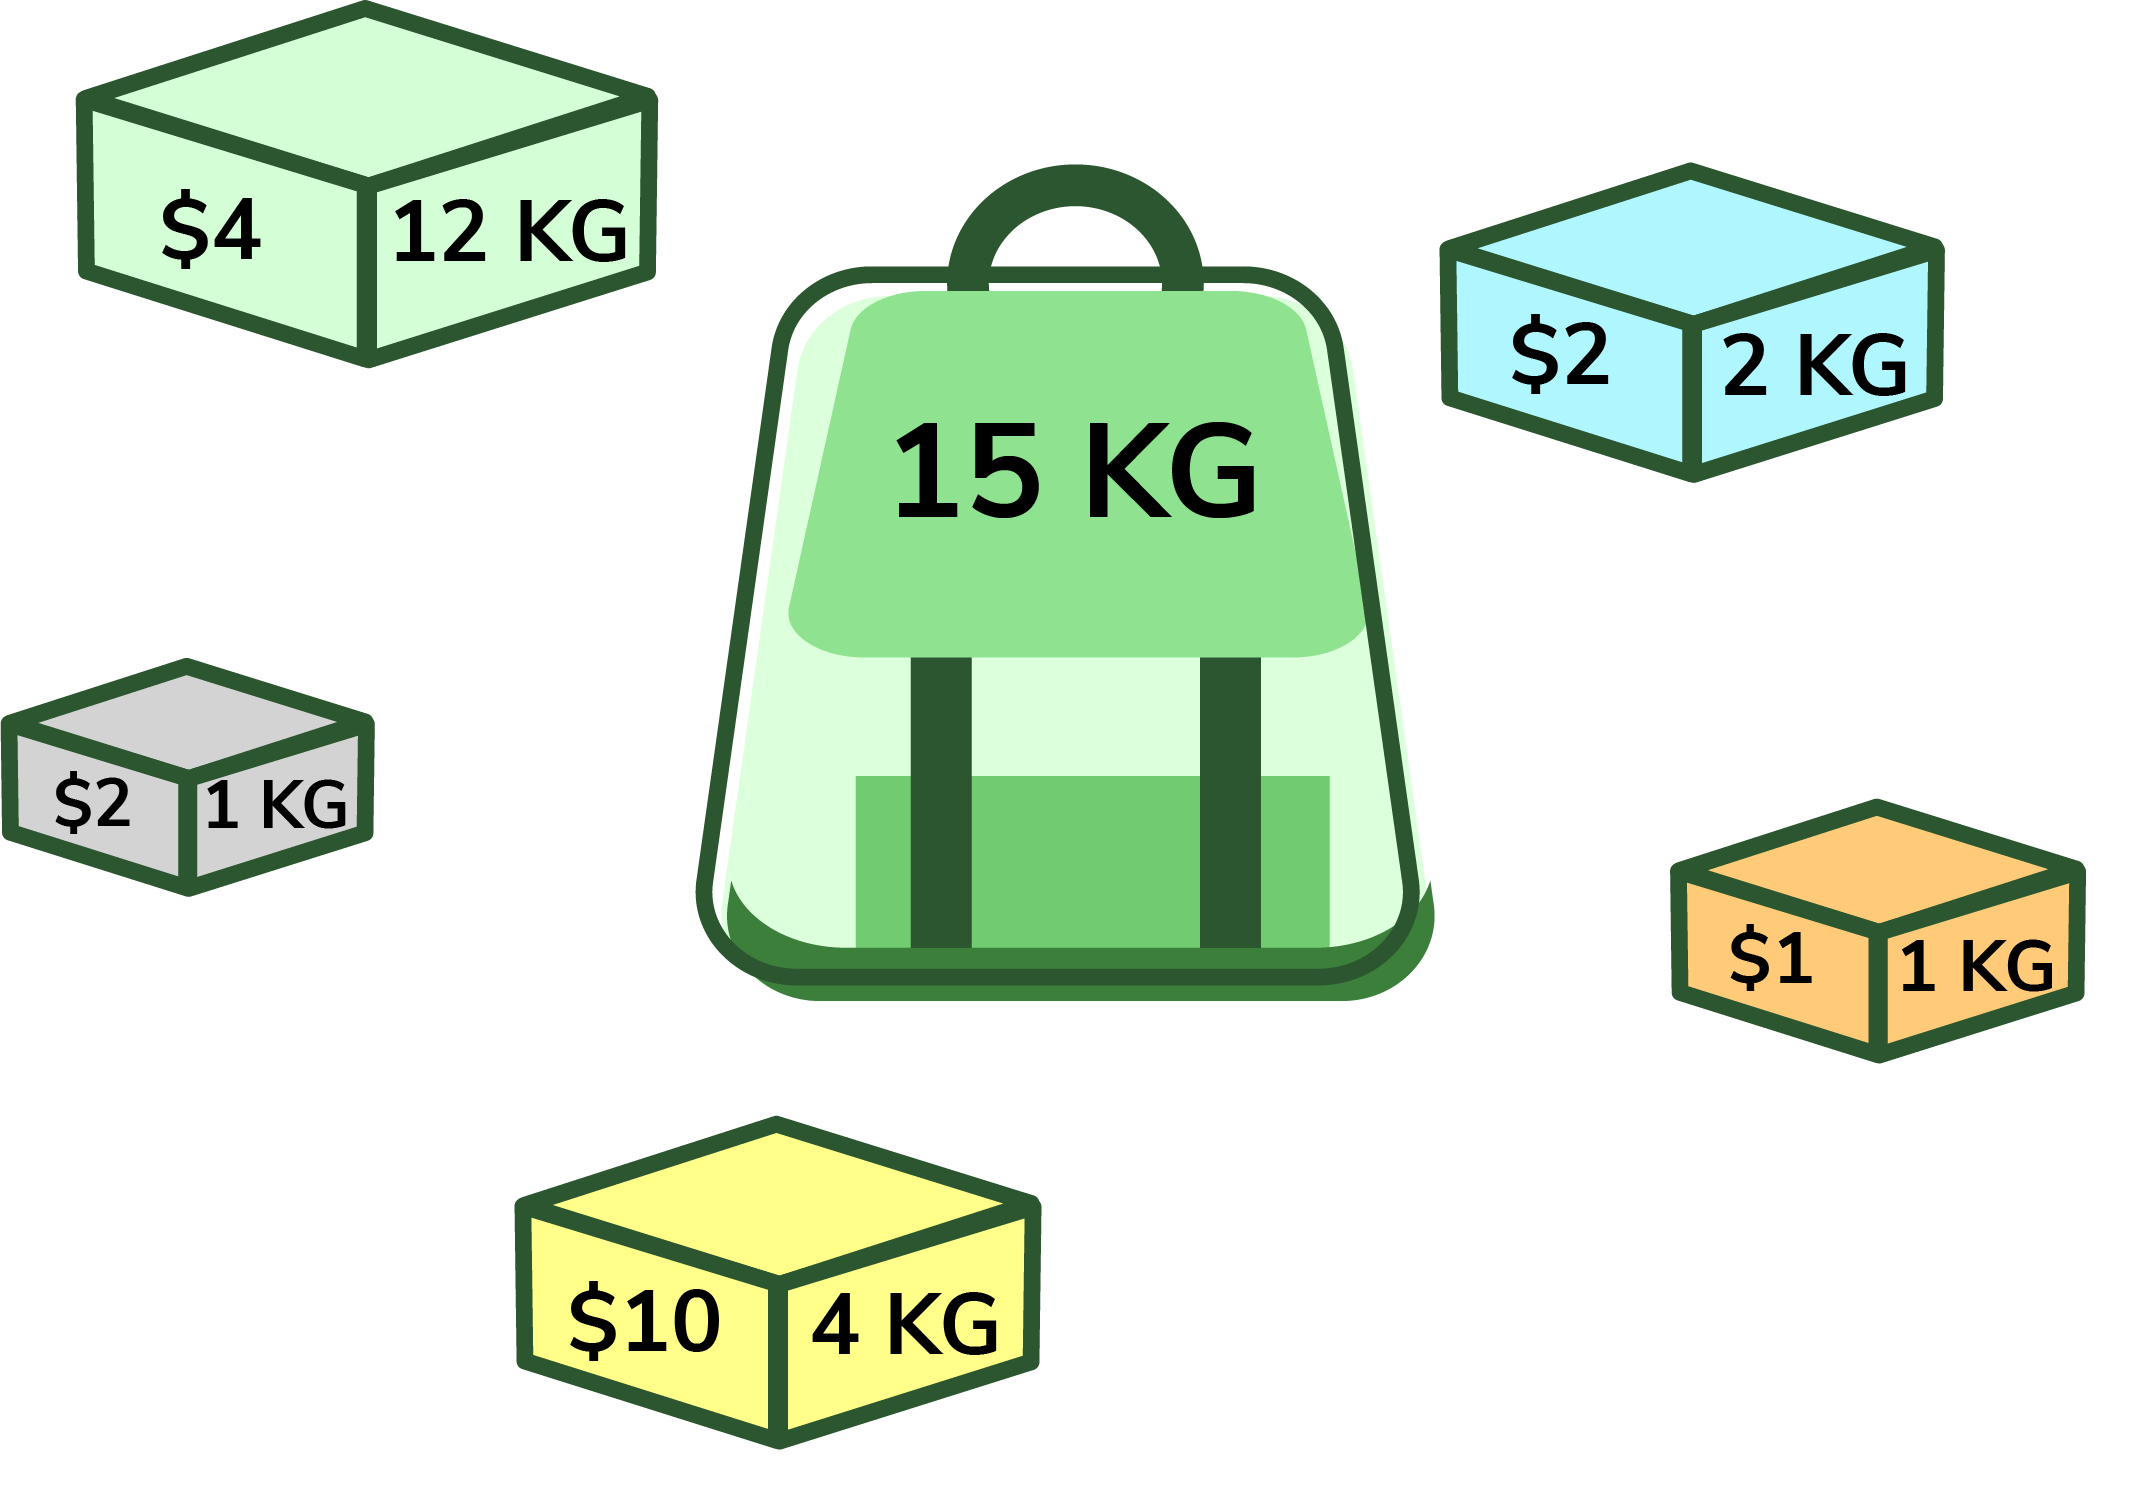
\includegraphics[width=0.9\textwidth, height=0.35\textheight]{knapsack_def.png}
                    \label{fig:knapsack_def}
                }
                
                \vspace{-1em} % Adjust space between the two images
                
                % Second subfigure (Venn Diagram)
                \subfloat[Computational Complexity Classes.]{
                    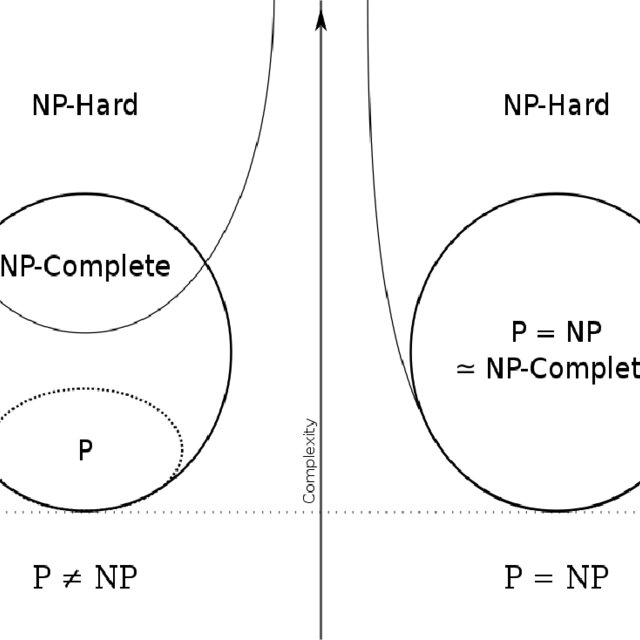
\includegraphics[width=0.9\textwidth, height=0.35\textheight]{np-venn.jpg}
                    \label{fig:np-venn}
                }
                
            \end{figure}
        \end{column}
        
        % --- RIGHT COLUMN: Definition and Importance ---
        \begin{column}{0.6\textwidth}
            
            % --- Top Part: The Definition ---
            \begin{block}{The 0/1 Knapsack Problem}
                Given $n$ items with weights and values, choose a subset.
                \begin{itemize}
                    \item \textbf{Objective:} Maximize the total value.
                    \item \textbf{Constraint:} The total weight must not exceed the knapsack's capacity.
                    \item \textbf{Rule:} Each item is either taken (1) or left (0), no fractions
                \end{itemize}
            \end{block}

            % --- Bottom Part: Context and Importance ---
            \begin{alertblock}{Applications \& Complexity}
                \begin{itemize}
                    \item \textbf{Real-world Applications:} Portfolio selection, resource allocation, logistics. \vspace{0.5em}
                    
                    \item \textbf{Problem Variants:} Many variants exist by altering constraints or item properties. The 0/1 version is the most common. \vspace{0.5em}
                    
                    \item \textbf{Computational Hardness:} KP is \textbf{NP-complete}. There is no known polynomial-time exact solution.
                \end{itemize}
            \end{alertblock}
            
        \end{column}
    \end{columns}
\end{frame}
% \section{Related Work \& My Contributions}

% \begin{frame}
%     \frametitle{Related Work: A Comparative Overview}

%     \begin{tiny} % Use tiny font size for this very dense table
%     \begin{tabular}{@{}llp{2.8cm}p{3cm}l@{}}
%     \toprule
%     \textbf{Work (Author, Year)} & \textbf{Architecture} & \textbf{Algorithm / Approach} & \textbf{Scalability / Generalization} & \textbf{Problem Domain} \\
%     \midrule
%     \multicolumn{5}{l}{\textit{\textbf{Foundational Pointer Network \& RL Models}}} \\
%     \addlinespace
%     Vinyals et al. (2015) & Pointer Network & Supervised Learning & Fixed-scale & TSP, Convex Hull \\
%     \addlinespace
%     Bello et al. (2017) & Pointer Network & RL (REINFORCE) & Fixed-scale (Train/Test on same size) & TSP, **Knapsack** \\
    
%     \addlinespace
%     \midrule
%     \addlinespace
    
%     \multicolumn{5}{l}{\textit{\textbf{Advanced Attention \& Transformer-based Models}}} \\
%     \addlinespace
%     Kool et al. (2019) & Transformer & RL (REINFORCE) & Fixed-scale & TSP, CVRP, **Knapsack** \\
%     \addlinespace
%     Yildiz (2022) & Transformer/Attn & RL (DQN) & Fixed-scale & **Knapsack** \\
%     \addlinespace
%     Gholipour et al. (2023) & Transformer & RL (PPO) & Fixed-scale & Task Offloading \\
    
%     \addlinespace
%     \midrule
%     \addlinespace
    
%     \rowcolor{blue!10} % Highlight your work
%     \textbf{Our Work} & \textbf{Custom (CNN+Attn)} & \textbf{RL (PPO-based)} & \textbf{Generalizes to larger scales} & \textbf{0/1 Knapsack} \\
    
%     \bottomrule
%     \end{tabular}
%     \end{tiny}
    
%     \vspace{1em}
%     \small % Return to a slightly larger font for the summary
%     \textbf{Key Limitations of Prior Work:} Most existing models are trained and tested on fixed-size problems, lacking generalization to different or larger scales.
    
% \end{frame}

\section{Related Work \& My Contributions}

\begin{frame}
    \frametitle{Related Work: A Comparative Overview}

    \begin{tiny} % Use tiny font size for this very dense table
    \begin{tabular}{@{}llp{2.8cm}p{3.6cm}l@{}}
    \toprule
    \textbf{Work (Author, Year)} & \textbf{Architecture} & \textbf{Algorithm / Approach} & \textbf{Scalability / Generalization} & \textbf{Problem Domain} \\
    \midrule
    \multicolumn{5}{l}{\textit{\textbf{Foundational Pointer Network \& RL Models (Often Lack Generalization)}}} \\
    \addlinespace
    Vinyals et al. (2015) & Pointer Network & Supervised Learning (Constructive) & Fixed-scale (Train and test on same small sizes) & TSP, Convex Hull \\
    \addlinespace
    Bello et al. (2017) & Pointer Network & RL (REINFORCE) (Constructive) & Fixed-scale (e.g., trained on N=50, tested on N=50) & TSP, **Knapsack** \\
    
    \addlinespace
    \midrule
    \addlinespace
    
    \multicolumn{5}{l}{\textit{\textbf{GNN-based and Hybrid Models (Often Generalize Better)}}} \\
    \addlinespace
    Dai et al. (2017) & GNN (structure2vec) & RL (DQN) (Constructive) & Generalizes to unseen \& larger scale graphs due to graph-based nature & MVC, MAXCUT, TSP \\
    \addlinespace
    Cappart et al. (2021) & DRL + CP (Hybrid) & DRL learns a heuristic for a Constraint Programming (CP) solver (Improvement) & Generalizes well to new, unseen instances of various sizes & TSPTW, **Knapsack** \\
    
    \addlinespace
    \midrule
    \addlinespace
    
    \multicolumn{5}{l}{\textit{\textbf{Advanced Transformer-based Models (Mixed Generalization)}}} \\
    \addlinespace
    Kool et al. (2019) & Transformer & RL (REINFORCE) (Constructive) & Generalizes to larger scales (e.g., train N=50, test N=100), but performance may degrade & TSP, CVRP \\
    \addlinespace
    Yildiz (2022) & Transformer/Attn & RL (DQN) (Constructive) & Fixed-scale (Performance degrades significantly on different sizes) & **Knapsack** \\
    \addlinespace
    Que et al. (2023) & Transformer & RL (PPO) (Constructive) & Fixed-scale (Trained and tested on same N) & 3D Packing \\
    \addlinespace
    Zhang et al. (2025) & Dueling DQN & RL (Dueling DQN) with state modification (Constructive) & Fixed-scale (Trained and tested on specific small sizes) & \textbf{0/1 Knapsack} \\

    \addlinespace
    \midrule
    \addlinespace
    
    \rowcolor{green!15} % Highlight your work
    \textbf{My Work} & \textbf{Custom Arch. + PPO} & \textbf{RL (PPO) (Constructive)} & \textbf{Generalizes to larger scales (Train on N, Test on >N with ~70\% acc.)} & \textbf{0/1 Knapsack} \\
    
    \bottomrule
    \end{tabular}
    \end{tiny}
    
    \vspace{0.1em}
    \footnotesize
    \textbf{My Contribution:} My work addresses a key limitation of many prior models by building a \textbf{generalizable framework}. Unlike fixed-scale approaches, our model is trained to solve knapsack problems of varying sizes, including those larger than seen during training, and is supported by a powerful, integrated platform for research.
    
\end{frame}
% ===================================================================
% SECTION 3: METHODOLOGY
% ===================================================================
\section{Methodology}

% --- Subsection 3.1: Algorithms ---
\subsection{Algorithms}

% --- Slide 1 ---
\begin{frame}
    \frametitle{Scalability Limits of Traditional \& Commercial Solvers}

    \begin{columns}[T]
        
        % --- LEFT COLUMN: Traditional Exact Algorithms ---
        \begin{column}{0.5\textwidth}
            \begin{block}{1. Space Complexity}
                \begin{figure}
                    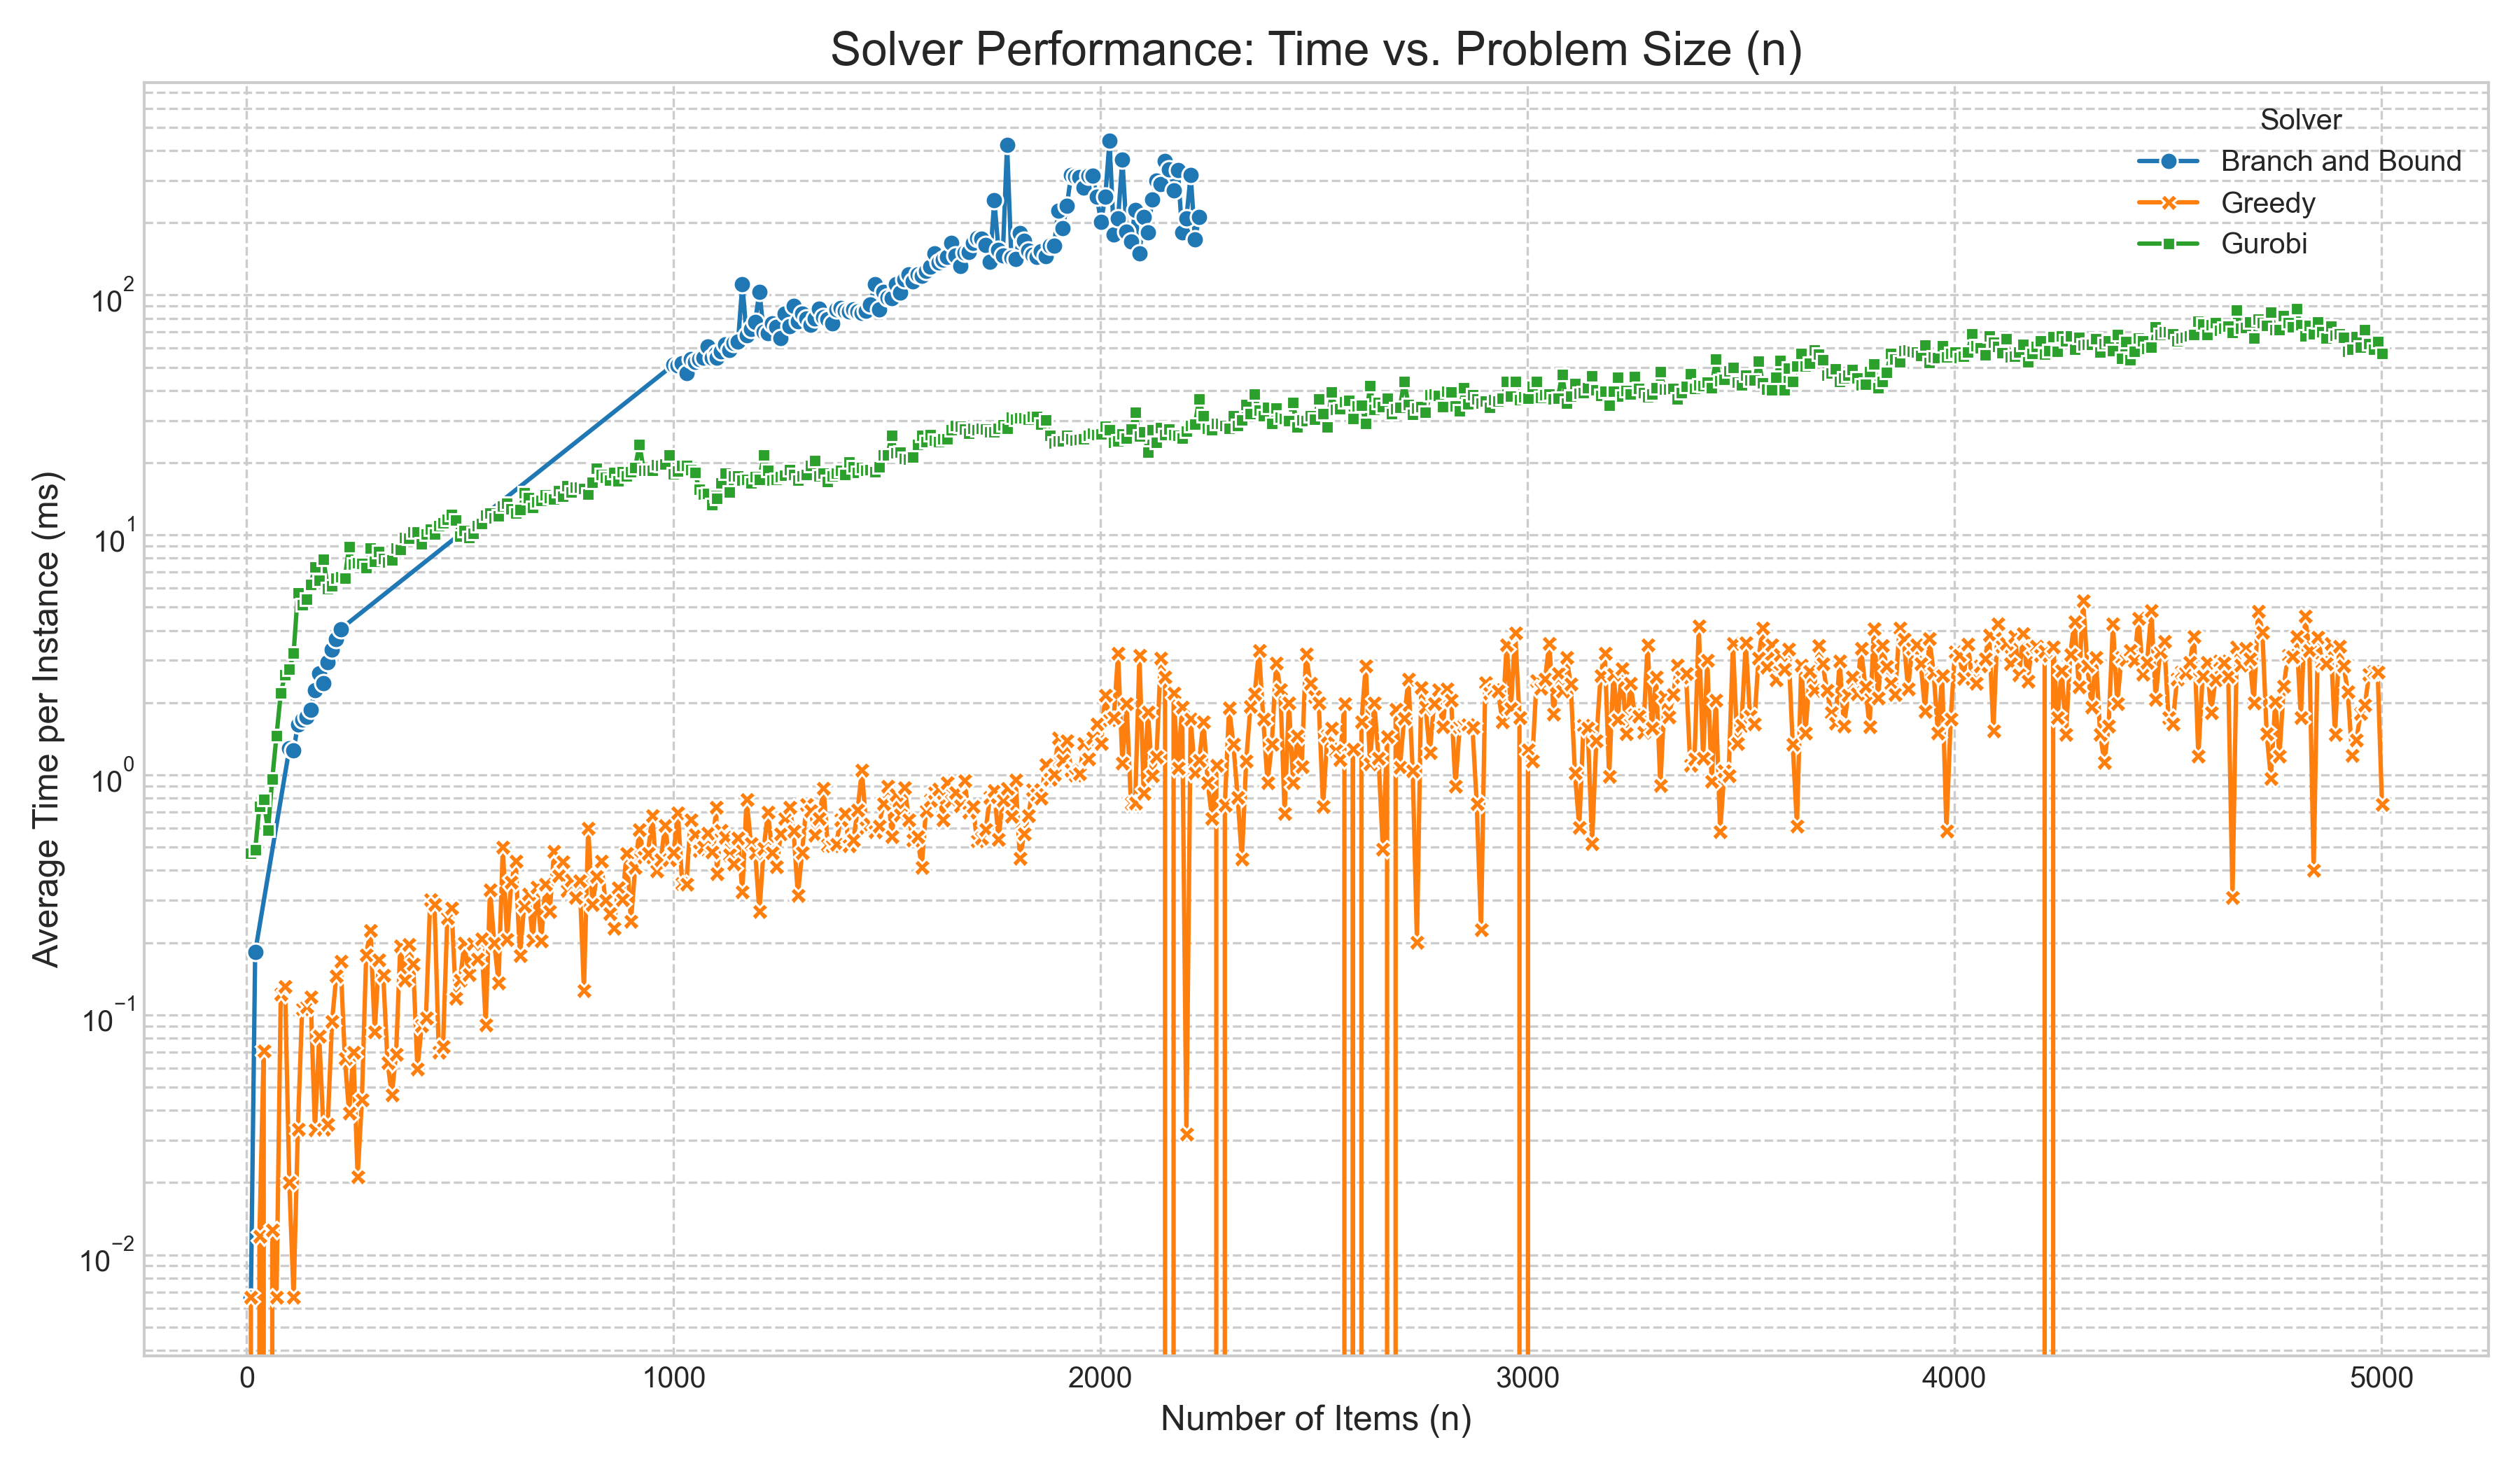
\includegraphics[width=\textwidth]{memory-explosion.png} 
                    \caption{Performance degradation due to memory constraints.}
                \end{figure}
                \vspace{-1.2em}
                \begin{itemize}
                    \item Suffer from the "curse of dimensionality".
                    \item Leads to a \textbf{memory explosion}, making them infeasible for large-scale problems.
                \end{itemize}
            \end{block}
        \end{column}

        % --- RIGHT COLUMN: Commercial Solvers ---
        \begin{column}{0.5\textwidth}
            \begin{block}{2. Time Complexity}
                \begin{figure}
                    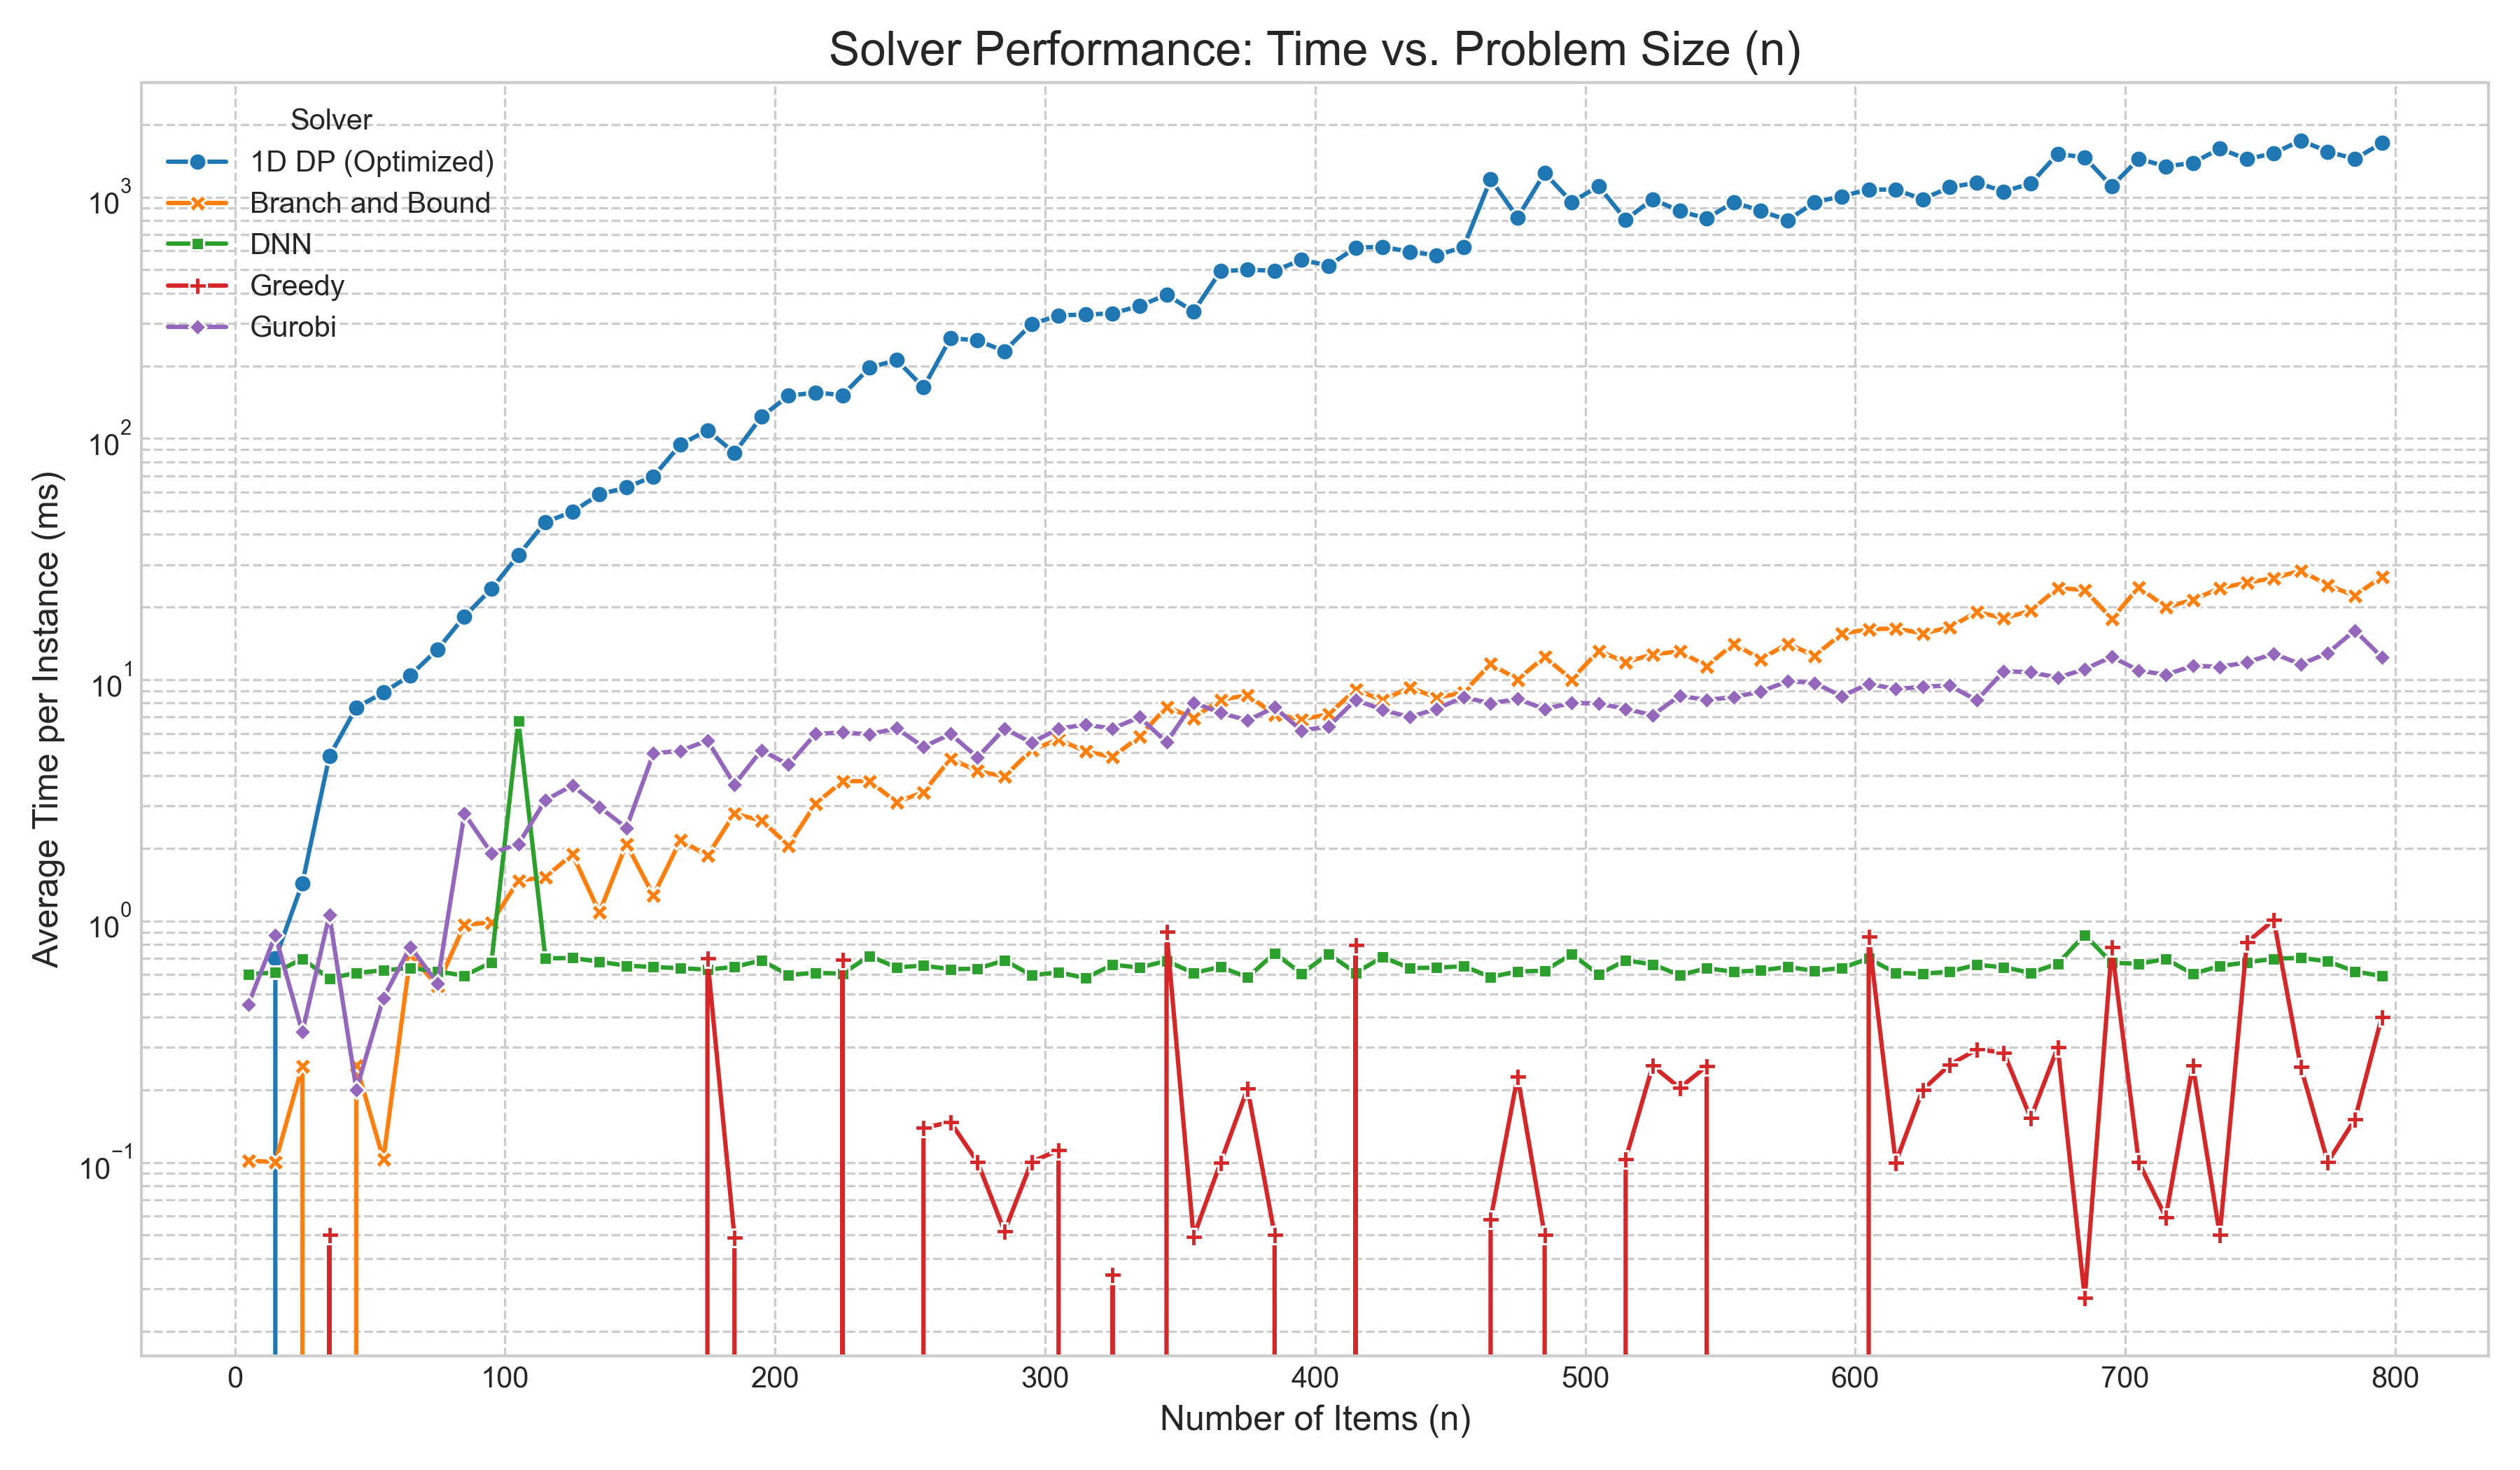
\includegraphics[width=\textwidth]{time-growth.png}
                    \caption{Performance comparison of various solvers.}
                \end{figure}
                \vspace{-1.2em}
                \begin{itemize}
                    \item Runtime of Commercial Solver like Gurobi still exhibits \textbf{exponential growth}, becoming a bottleneck for very large problems.
                \end{itemize}
            \end{block}
        \end{column}

    \end{columns}
\end{frame}

% --- SLIDE 2: RL Fundamentals & Bellman Equation ---
\begin{frame}
    \frametitle{RL Fundamentals \& The Bellman Equation}

    \begin{columns}[T]
        
        % --- LEFT COLUMN: RL Components for the 0/1 Knapsack Problem ---
        \begin{column}{0.5\textwidth}
            \begin{block}{Key RL Components for 0/1 KP}
                \begin{itemize}
                    \item \textbf{State ($s_t$):} The set of available items and the current remaining knapsack capacity. \vspace{0.5em}
                    
                    \item \textbf{Action ($a_t$):} The selection of one item from the available set that fits the capacity. \vspace{0.5em}
                    
                    \item \textbf{Policy ($\pi_\theta(a|s)$):} A neural network that maps the current state to a probability distribution over valid actions (items to select). \vspace{0.5em}
                    
                    \item \textbf{Reward ($R_{t+1}$):} The value ($v_i$) of the selected item. \vspace{0.5em}
                    
                    \item \textbf{Episode ($\tau$):} A sequence of item selections, ending when no more items can be legally packed.
                \end{itemize}
            \end{block}
        \end{column}
        
        % --- RIGHT COLUMN: Two Forms of the Bellman Equation ---
        \begin{column}{0.5\textwidth}
            
            \begin{alertblock}{1. Bellman Expectation Equation (Policy-based)}
                Calculates the value function $\mathbf{v}^\pi$ for a \textbf{given policy $\pi$}.
                \begin{align*}
                    \mathbf{v}^{\pi} = \mathbf{r}^{\pi} + \gamma \mathbf{P}^{\pi} \mathbf{v}^{\pi}
                \end{align*}
                This is the foundation for the \textbf{Critic} in Actor-Critic methods like PPO, which evaluates the current policy.
            \end{alertblock}
            
            \vspace{1em}

            \begin{block}{2. Bellman Optimality Equation (Value-based)}
                Defines the optimal value function $\mathbf{v}^*$ by finding the best action at each state.
                \begin{align*}
                    \mathbf{v}^{*} = \max_{a} \left( \mathbf{r}(a) + \gamma \mathbf{P}(a) \mathbf{v}^{*} \right)
                \end{align*}
                This is the target for value-based methods like Q-Learning, which directly learn the optimal policy.
            \end{block}

        \end{column}

    \end{columns}
\end{frame}

% --- Slide 3: REINFORCE Algorithm and Architecture ---
\begin{frame}
    \frametitle{REINFORCE: Algorithm and Architecture}

    \begin{columns}[T]
        
        % --- LEFT COLUMN: Algorithm Flowchart ---
        \begin{column}{0.5\textwidth}
            \begin{block}{Training Algorithm}
                \begin{figure}
                    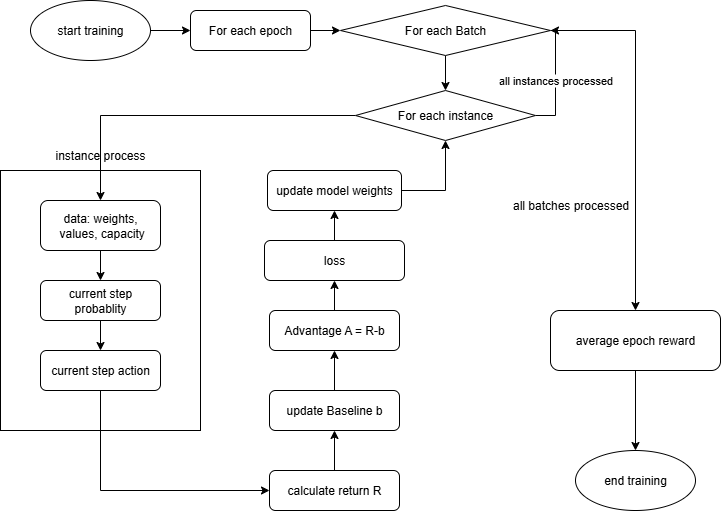
\includegraphics[width=\textwidth]{reinforce_training_manual.png}
                    \caption{The REINFORCE training loop with an EMA baseline.}
                \end{figure}

                \vspace{-1.5em}

                \begin{itemize}
                    % \item An entire episode (trajectory) is sampled per update.
                    \item The policy is updated based on the total return of the episode.
                    \item A baseline is used to reduce gradient variance.
                \end{itemize}
            \end{block}
        \end{column}

        % --- RIGHT COLUMN: Model Architecture ---
        \begin{column}{0.5\textwidth}
            \begin{block}{Model Architecture}
                \begin{figure}
                    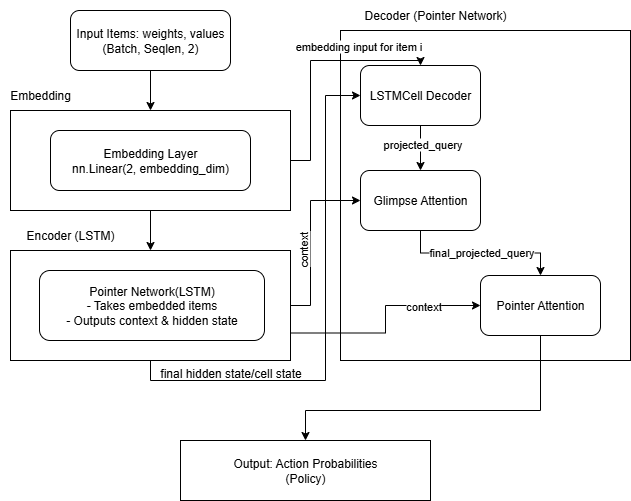
\includegraphics[width=\textwidth]{ptrn_arch.png}
                    \caption{Pointer Network-based architecture for sequential item selection.}
                \end{figure}
                \vspace{-1.5em}
                \begin{itemize}
                    \item One Actor and no Critic.
                \end{itemize}
            \end{block}
        \end{column}

    \end{columns}
\end{frame}

% --- Slide 4: PPO Algorithm and Model Architecture ---
\begin{frame}
    \frametitle{PPO: Algorithm and Architecture}

    \begin{columns}[T]
        \vspace{-1em}
        
        % --- LEFT COLUMN: PPO Algorithm Flowchart ---
        \begin{column}{0.5\textwidth}
            \begin{block}{Training Algorithm}
                \begin{figure}
                    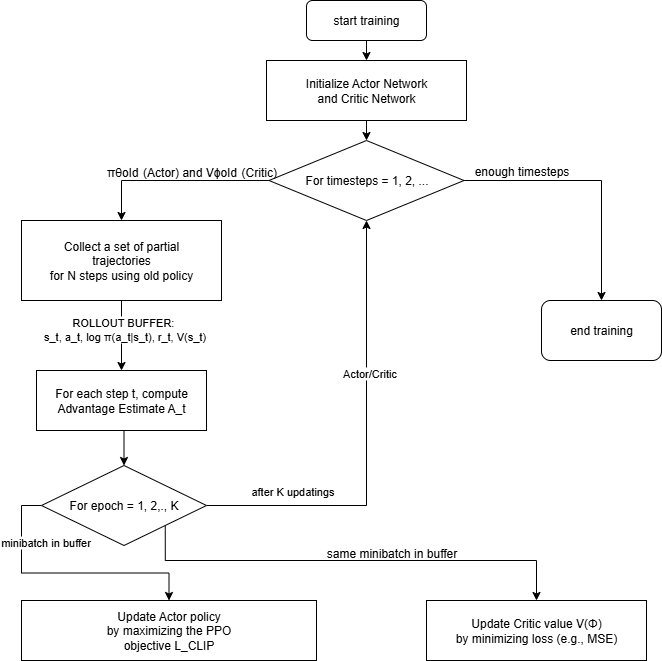
\includegraphics[width=0.85\textwidth, height=0.63\textheight]{PPO_training_manual.png}
                    \caption{The PPO training loop using an Actor-Critic framework.}
                \end{figure}
                \vspace{-1.5em}
                \begin{itemize}
                    \item Multiple optimization on the same minibatch.
                \end{itemize}
            \end{block}
        \end{column}

        % --- RIGHT COLUMN: PPO Model Architecture ---
        \begin{column}{0.5\textwidth}
            \begin{block}{Model Architecture}
                \begin{figure}
                    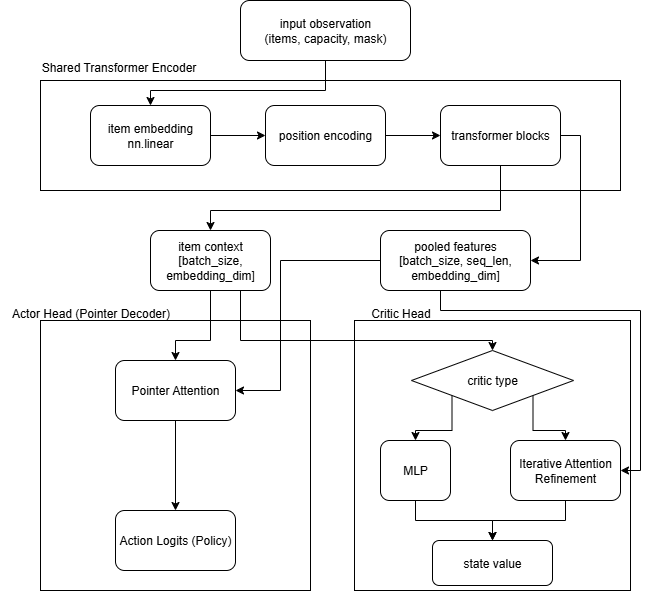
\includegraphics[width=0.85\textwidth, height=0.6\textheight]{ppo_model_manual.png}
                    \caption{The model has two heads: one for the policy (Actor) and one for the value (Critic).}
                \end{figure}
                \vspace{-1.5em}
                \begin{itemize}
                    \item Actor and Critic share the same encoder.
                    % \item The Actor outputs a probability distribution over actions (items).
                    % \item The Critic outputs a value estimate for the current state.
                \end{itemize}
            \end{block}
        \end{column}

    \end{columns}
\end{frame}

% \begin{frame}
%     \frametitle{Algorithm Implementation: REINFORCE with Baseline}
    
%     % The algorithmic environment is for typesetting pseudocode
%     % The [1] adds line numbers
%     \begin{algorithmic}[1]
%         \State \textbf{Initialize:} Policy network $\pi_\theta$, optimizer, and EMA baseline $b \gets 0$.
%         \vspace{0.5em}
        
%         \For{each epoch}
%             \For{each batch of problems}
%                 \State // \textit{1. Rollout Phase}
%                 \State Sample trajectories $\{\tau_1, \tau_2, ...\}$ using the current policy $\pi_\theta$.
%                 \vspace{0.5em}
                
%                 \State // \textit{2. Advantage Calculation}
%                 \State Compute returns $R(\tau_i)$ for each trajectory (total packed value).
%                 \State Update EMA baseline: $b \gets \beta \cdot b + (1-\beta) \cdot \text{mean}(R)$.
%                 \State Calculate advantage for each trajectory: $\hat{A}(\tau_i) \gets R(\tau_i) - b$.
%                 \vspace{0.5em}
                
%                 \State // \textit{3. Policy Update}
%                 \State Calculate policy loss: $\mathcal{L}(\theta) \gets - \frac{1}{N}\sum_{i} \log p_\theta(\tau_i) \cdot \hat{A}(\tau_i)$.
%                 \State Update policy network parameters $\theta$ via backpropagation.
%             \EndFor
%         \EndFor
%     \end{algorithmic}
    
%     \vfill % Pushes the block to the bottom
    
%     \begin{alertblock}{Key Idea}
%         An Exponential Moving Average (EMA) baseline ($b$) is subtracted from the return ($R$) to calculate the \textbf{advantage} ($\hat{A}$). This significantly reduces the variance of the policy gradient, leading to more stable and faster training.
%     \end{alertblock}

% \end{frame}

% % --- Slide 2: Choosing the Right Reinforcement Learning Approach ---
% \begin{frame}
%     \frametitle{Choosing the Right Reinforcement Learning Approach}

%     \begin{columns}[T]
        
%         % --- LEFT COLUMN: Policy-based vs. Value-based ---
%         \begin{column}{0.5\textwidth}
%             \begin{block}{Value-based Methods (e.g., DQN)}
%                 \begin{itemize}
%                     \item \textbf{What it learns:} A value function $Q(s, a)$ that estimates the max future reward.
%                     \item \textbf{How it acts:} Chooses the action with the highest estimated value.
%                     \item \textbf{Limitation:} Can be inefficient or unstable in large/continuous action spaces, as is the case for KP with many items.
%                 \end{itemize}
%             \end{block}

%             \begin{alertblock}{Policy-based Methods (Our Choice)}
%                 \begin{itemize}
%                     \item \textbf{What it learns:} Directly learns a policy $\pi(a|s)$, a probability distribution over actions.
%                     \item \textbf{How it acts:} Samples an action directly from the policy.
%                     \item \textbf{Advantage:} More effective for complex action spaces and can learn stochastic policies, which aids exploration.
%                 \end{itemize}
%             \end{alertblock}
%         \end{column}

%         % --- RIGHT COLUMN: MC vs. TD updates ---
%         \begin{column}{0.5\textwidth}
%             \begin{block}{Monte Carlo Updates (e.g., REINFORCE)}
%                 \begin{itemize}
%                     \item \textbf{How it updates:} Waits until an entire episode is finished, then updates the policy based on the final total reward.
%                     \item \textbf{Limitation:} High variance in updates because one good/bad final outcome is attributed to all actions taken, leading to unstable training.
%                 \end{itemize}
%             \end{block}
            
%             \begin{alertblock}{Temporal Difference (TD) Updates (PPO's basis)}
%                 \begin{itemize}
%                     \item \textbf{How it updates:} Updates the policy after each step (or a few steps), using a learned value estimate (from a Critic) to judge actions.
%                     \item \textbf{Advantage:} Lower variance and more sample-efficient as it learns from every step. PPO further improves stability with its clipped objective.
%                 \end{itemize}
%             \end{alertblock}
%         \end{column}

%     \end{columns}

%     \vfill % Pushes the summary to the bottom
%     \small\textit{Conclusion: Our framework uses PPO, a policy-based, Actor-Critic (TD) method, to leverage its stability and effectiveness in large action spaces.}
    
% \end{frame}

% % --- Slide 3: Policy Gradient Algorithm Formulas ---
% \begin{frame}
%     \frametitle{Policy Gradient Algorithms: REINFORCE vs. PPO}

%     \begin{columns}[T]
        
%         % --- LEFT COLUMN: REINFORCE ---
%         \begin{column}{0.5\textwidth}
%             \begin{block}{REINFORCE (Monte Carlo)}
%                 \textbf{Objective:} Maximize the expected total reward.
%                 \begin{align*}
%                     J(\theta) = \mathbb{E}_{\tau \sim \pi_\theta}[R(\tau)]
%                 \end{align*}
                
%                 \textbf{Policy Gradient:} The policy is updated using the gradient of the objective. The update rule relies on the full return $G_t$.
%                 \begin{align*}
%                      \nabla_\theta J(\theta) \propto \sum_{t=0}^{T} \nabla_\theta \log \pi_\theta(a_t|s_t) G_t 
%                 \end{align*}
                
%                 \textbf{Where:}
%                 \begin{itemize}
%                     \item $\pi_\theta(a_t|s_t)$ is the policy network.
%                     \item $G_t = \sum_{k=t}^{T} \gamma^{k-t} r_k$ is the total discounted reward from step $t$.
%                 \end{itemize}
%                 \textbf{Limitation:} High variance due to using the noisy full return $G_t$.
%             \end{block}
%         \end{column}

%         % --- RIGHT COLUMN: PPO ---
%         \begin{column}{0.5\textwidth}
%             \begin{alertblock}{PPO (Temporal Difference)}
%                 \textbf{Objective (Clipped Surrogate):} PPO constrains the policy change to improve stability.
%                 \begin{align*}
%                     L^{CLIP}(\theta) = \hat{\mathbb{E}}_t \Big[ \min \big( r_t(\theta)\hat{A}_t, \\ 
%                     \text{clip}(r_t(\theta), 1-\epsilon, 1+\epsilon) \hat{A}_t \big) \Big]
%                 \end{align*}
                
%                 \textbf{Where:}
%                 \begin{itemize}
%                     \item $r_t(\theta) = \frac{\pi_\theta(a_t|s_t)}{\pi_{\theta_{old}}(a_t|s_t)}$ is the probability ratio.
%                     \item $\hat{A}_t = G_t - V(s_t)$ is the \textbf{Advantage Estimate}, which has lower variance than $G_t$.
%                     \item $\epsilon$ is a hyperparameter for clipping.
%                 \end{itemize}
%                 \textbf{Advantage:} Stable, reliable, and sample-efficient.
%             \end{alertblock}
%         \end{column}

%     \end{columns}
% \end{frame}

% --- Subsection 3.2: Model Architecture ---
% \subsection{Model Architecture}

% % --- Slide 4: Overall Framework ---
% \begin{frame}
%     \frametitle{Our Proposed End-to-End RL Framework}
    
%     \begin{figure}
%         % --- Placeholder for your overall framework diagram ---
%         % --- e.g., a flowchart showing State -> Model -> Action -> Reward -> Update ---
%         \includegraphics[width=\textwidth]{placeholder.png}
%         \caption{The end-to-end process of solving a Knapsack instance using our PPO-based framework.}
%     \end{figure}

%     \begin{itemize}
%         \item Our framework takes a raw knapsack instance as input.
%         \item The \textbf{Actor-Critic} model outputs a policy for item selection.
%         \item The agent builds the solution sequentially.
%         \item The policy is updated using the \textbf{Proximal Policy Optimization (PPO)} algorithm.
%     \end{itemize}
% \end{frame}

% % --- Slide 5: Detailed Neural Network Architecture ---
% \begin{frame}
%     \frametitle{Detailed Model Architecture}
    
%     \begin{figure}
%         % --- Placeholder for your detailed neural network diagram ---
%         % --- e.g., showing input embeddings, CNN layers, attention, output heads ---
%         \includegraphics[width=\textwidth]{placeholder.png}
%         \caption{The internal architecture of our policy and value networks.}
%     \end{figure}

%     % --- You can use columns to describe different parts of the architecture ---
%     \begin{columns}[T]
%         \begin{column}{0.5\textwidth}
%             \textbf{Encoder:}
%             \begin{itemize}
%                 \item Processes the set of items.
%                 \item Captures relationships between items.
%             \end{itemize}
%         \end{column}
%         \begin{column}{0.5\textwidth}
%             \textbf{Decoder (Actor-Critic):}
%             \begin{itemize}
%                 \item Selects items sequentially.
%                 \item Outputs the action probability (policy) and state value.
%             \end{itemize}
%         \end{column}
%     \end{columns}
% \end{frame}
% ===================================================================
% SECTION 4: EXPERIMENTS & RESULTS
% ===================================================================
\section{Experiments \& Results}

% --- Subsection 4.1: Experimental Setup ---
\subsection{Experimental Setup}

% --- Slide 1: Dataset Generation ---
\begin{frame}
    \frametitle{Dataset Generation and Preprocessing}

    \begin{block}{Dataset Specification}
        We generated three distinct datasets for training, validation, and testing to ensure a robust evaluation of the model's generalization capabilities.
        
        \vspace{1em}
        \centering % Center the table
        \begin{tabular}{l c c c}
        \toprule
        \textbf{Parameter} & \textbf{Training Set} & \textbf{Validation Set} & \textbf{Test Set} \\
        \midrule
        Item Count Range ($n$) & 5 to 50 & 5 to 50 & \textbf{5 to 200} \\
        Step Size & 5 & 5 & 5 \\
        Instances per Size & 100 & 30 & 50 \\
        \addlinespace
        \textbf{Total Instances} & \textbf{1,000} & \textbf{300} & \textbf{1,950} \\
        \bottomrule
        \end{tabular}
    \end{block}
    
    \begin{columns}[T]
        \begin{column}{0.5\textwidth}
            \begin{alertblock}{Item Properties}
                \begin{itemize}
                    \item Weights ($w_i$) and values ($v_i$) are integers sampled uniformly from $U[1, 100]$.
                    \item There is no correlation between an item's weight and its value.
                    \item All inputs are normalized before being fed to the model.
                \end{itemize}
            \end{alertblock}
        \end{column}
        \begin{column}{0.5\textwidth}
            \begin{alertblock}{Problem Instance Constraints}
                \begin{itemize}
                    \item The knapsack capacity ($C$) is set relative to the total weight of all items ($\sum w_i$).
                    \item The ratio $\frac{C}{\sum w_i}$ is randomly sampled from $U[0.1, 0.9]$.
                \end{itemize}
            \end{alertblock}
        \end{column}
    \end{columns}
    
\end{frame}

% --- Subsection 4.2: Performance Results ---
\subsection{Performance Results}

% --- NEW Combined Slide for Accuracy and Speed Results ---
\begin{frame}
    \frametitle{Results: Accuracy and Inference Time}

    % --- TOP PART: Two figures side-by-side ---
    \begin{figure}
        \centering
        % Use subfloat for side-by-side figures with individual captions
        \subfloat[Mean Relative Error (MRE) vs. Problem Size.]{
            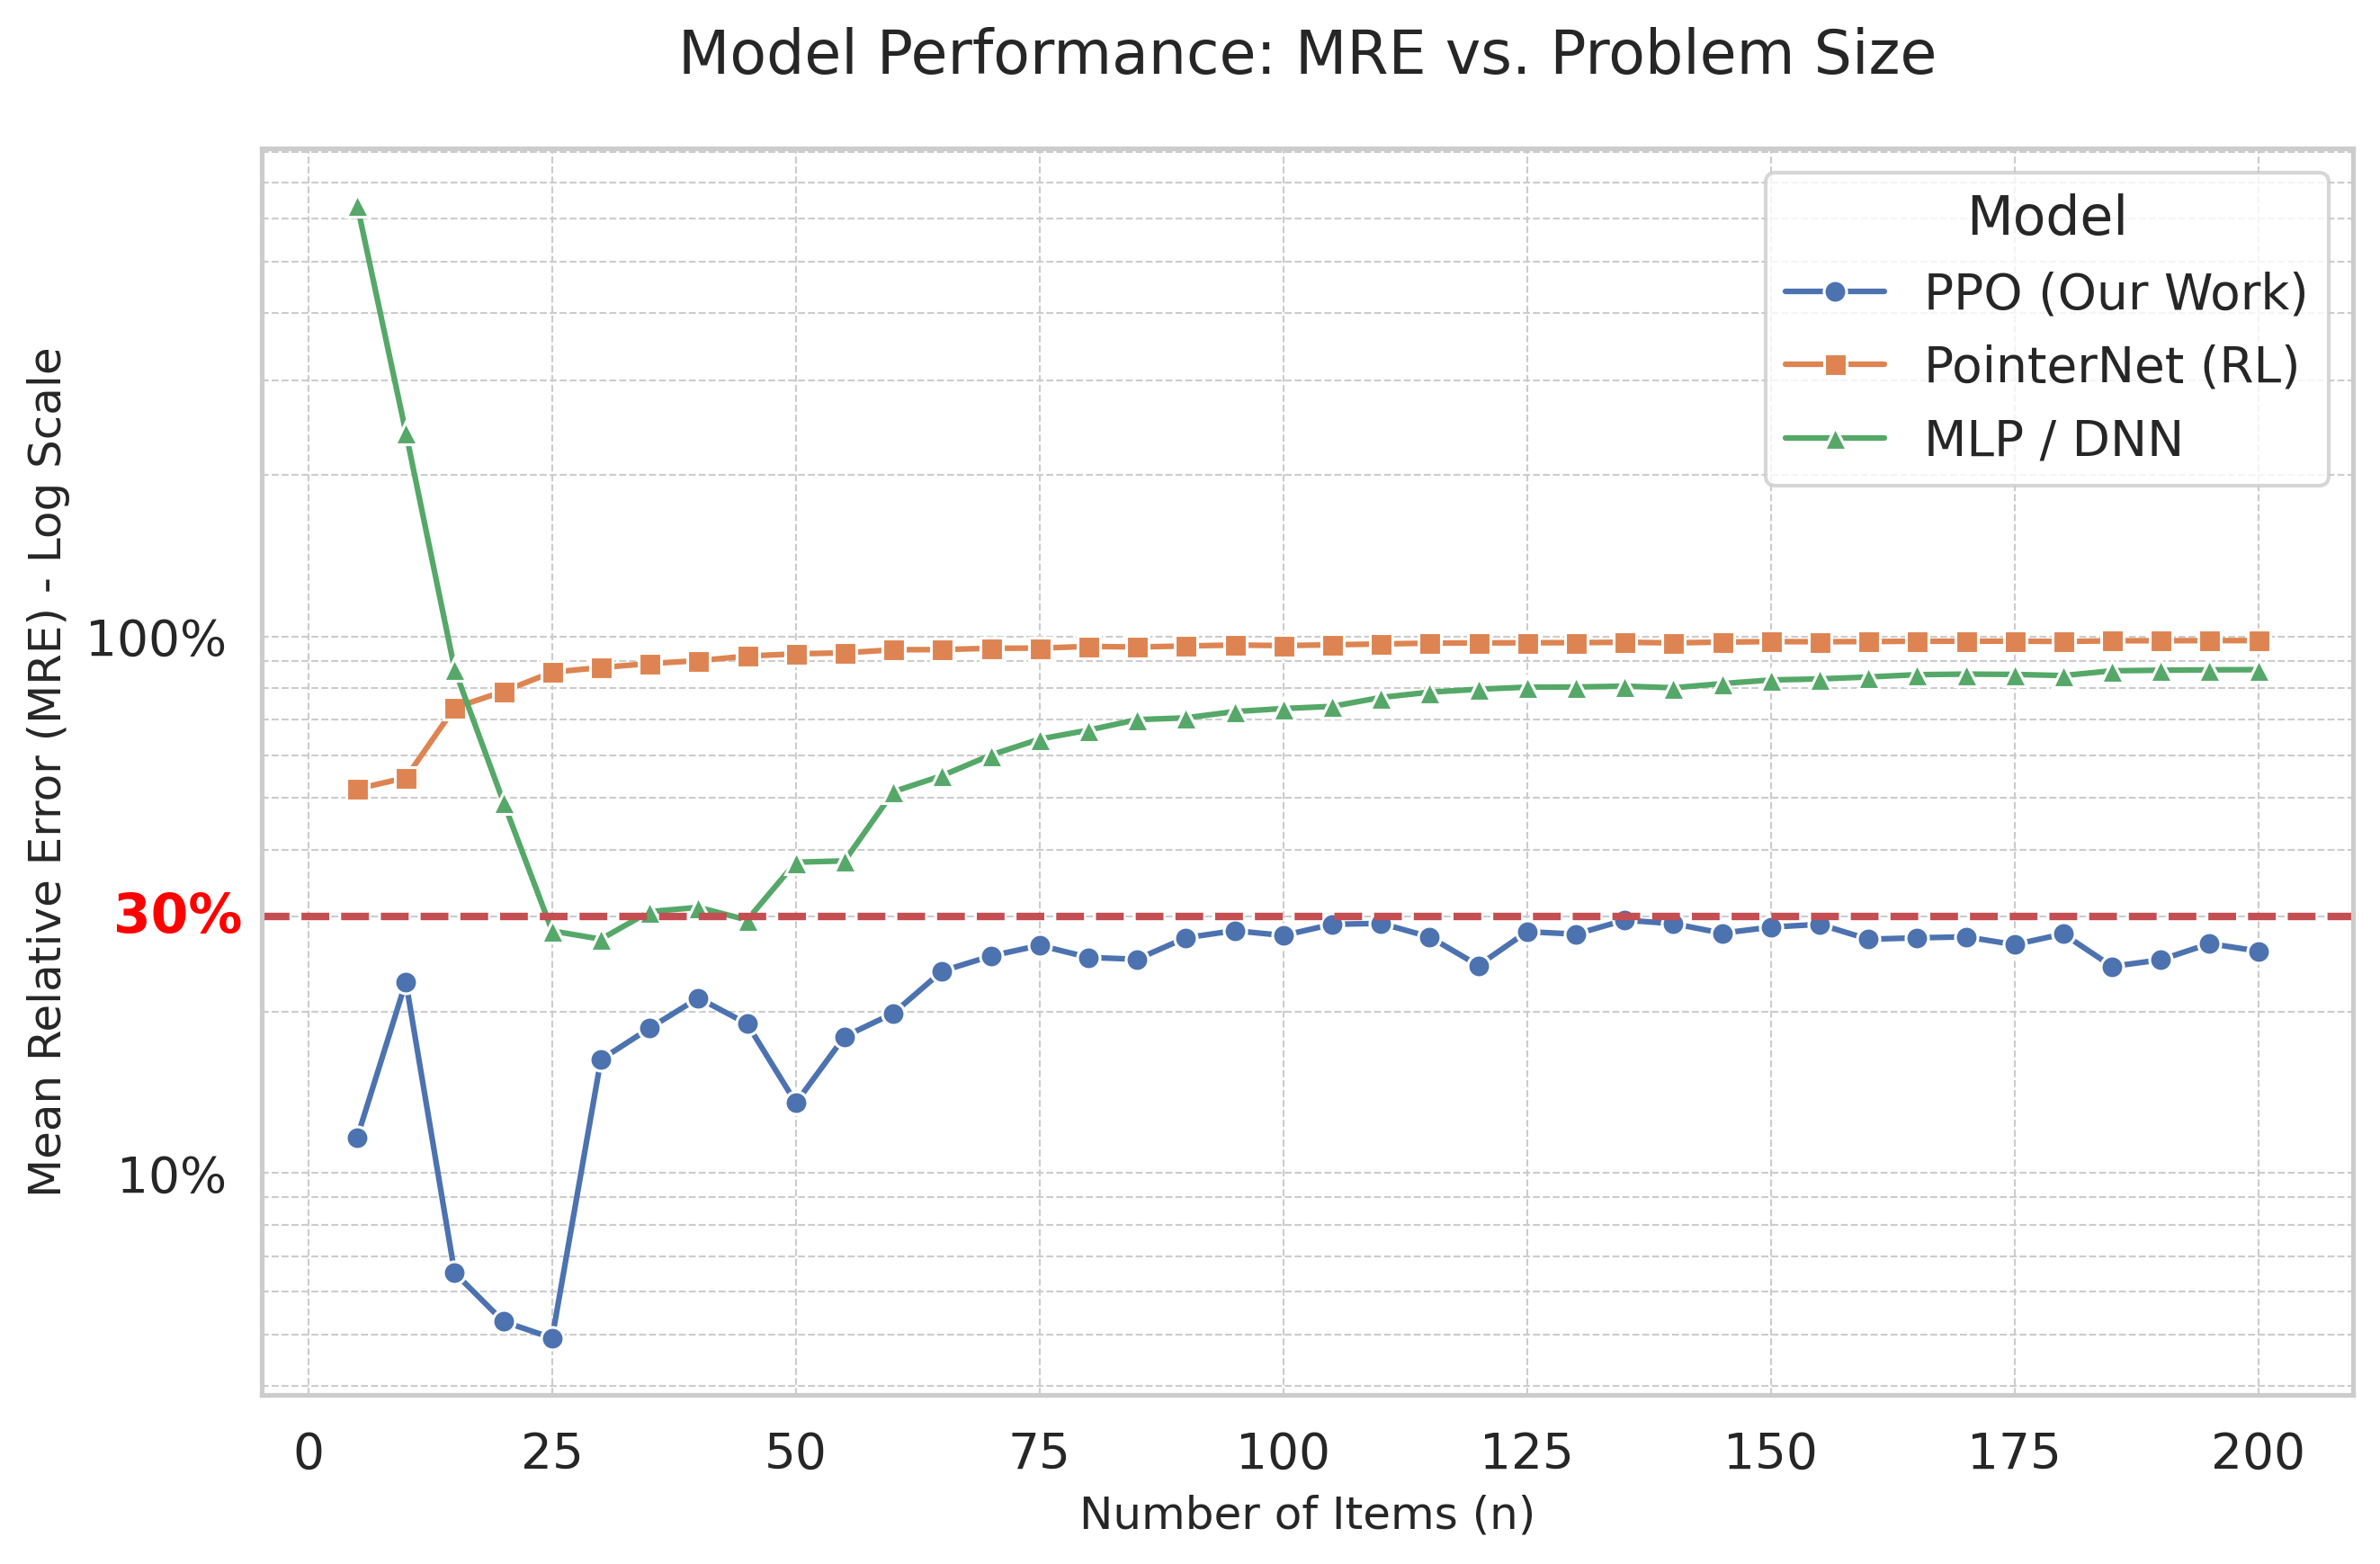
\includegraphics[width=0.48\textwidth]{mre_vs_problem_size_styled.png}
            \label{fig:mre_results}
        }
        \hfill % Creates a flexible space between the figures
        \subfloat[Inference Time vs. Problem Size.]{
            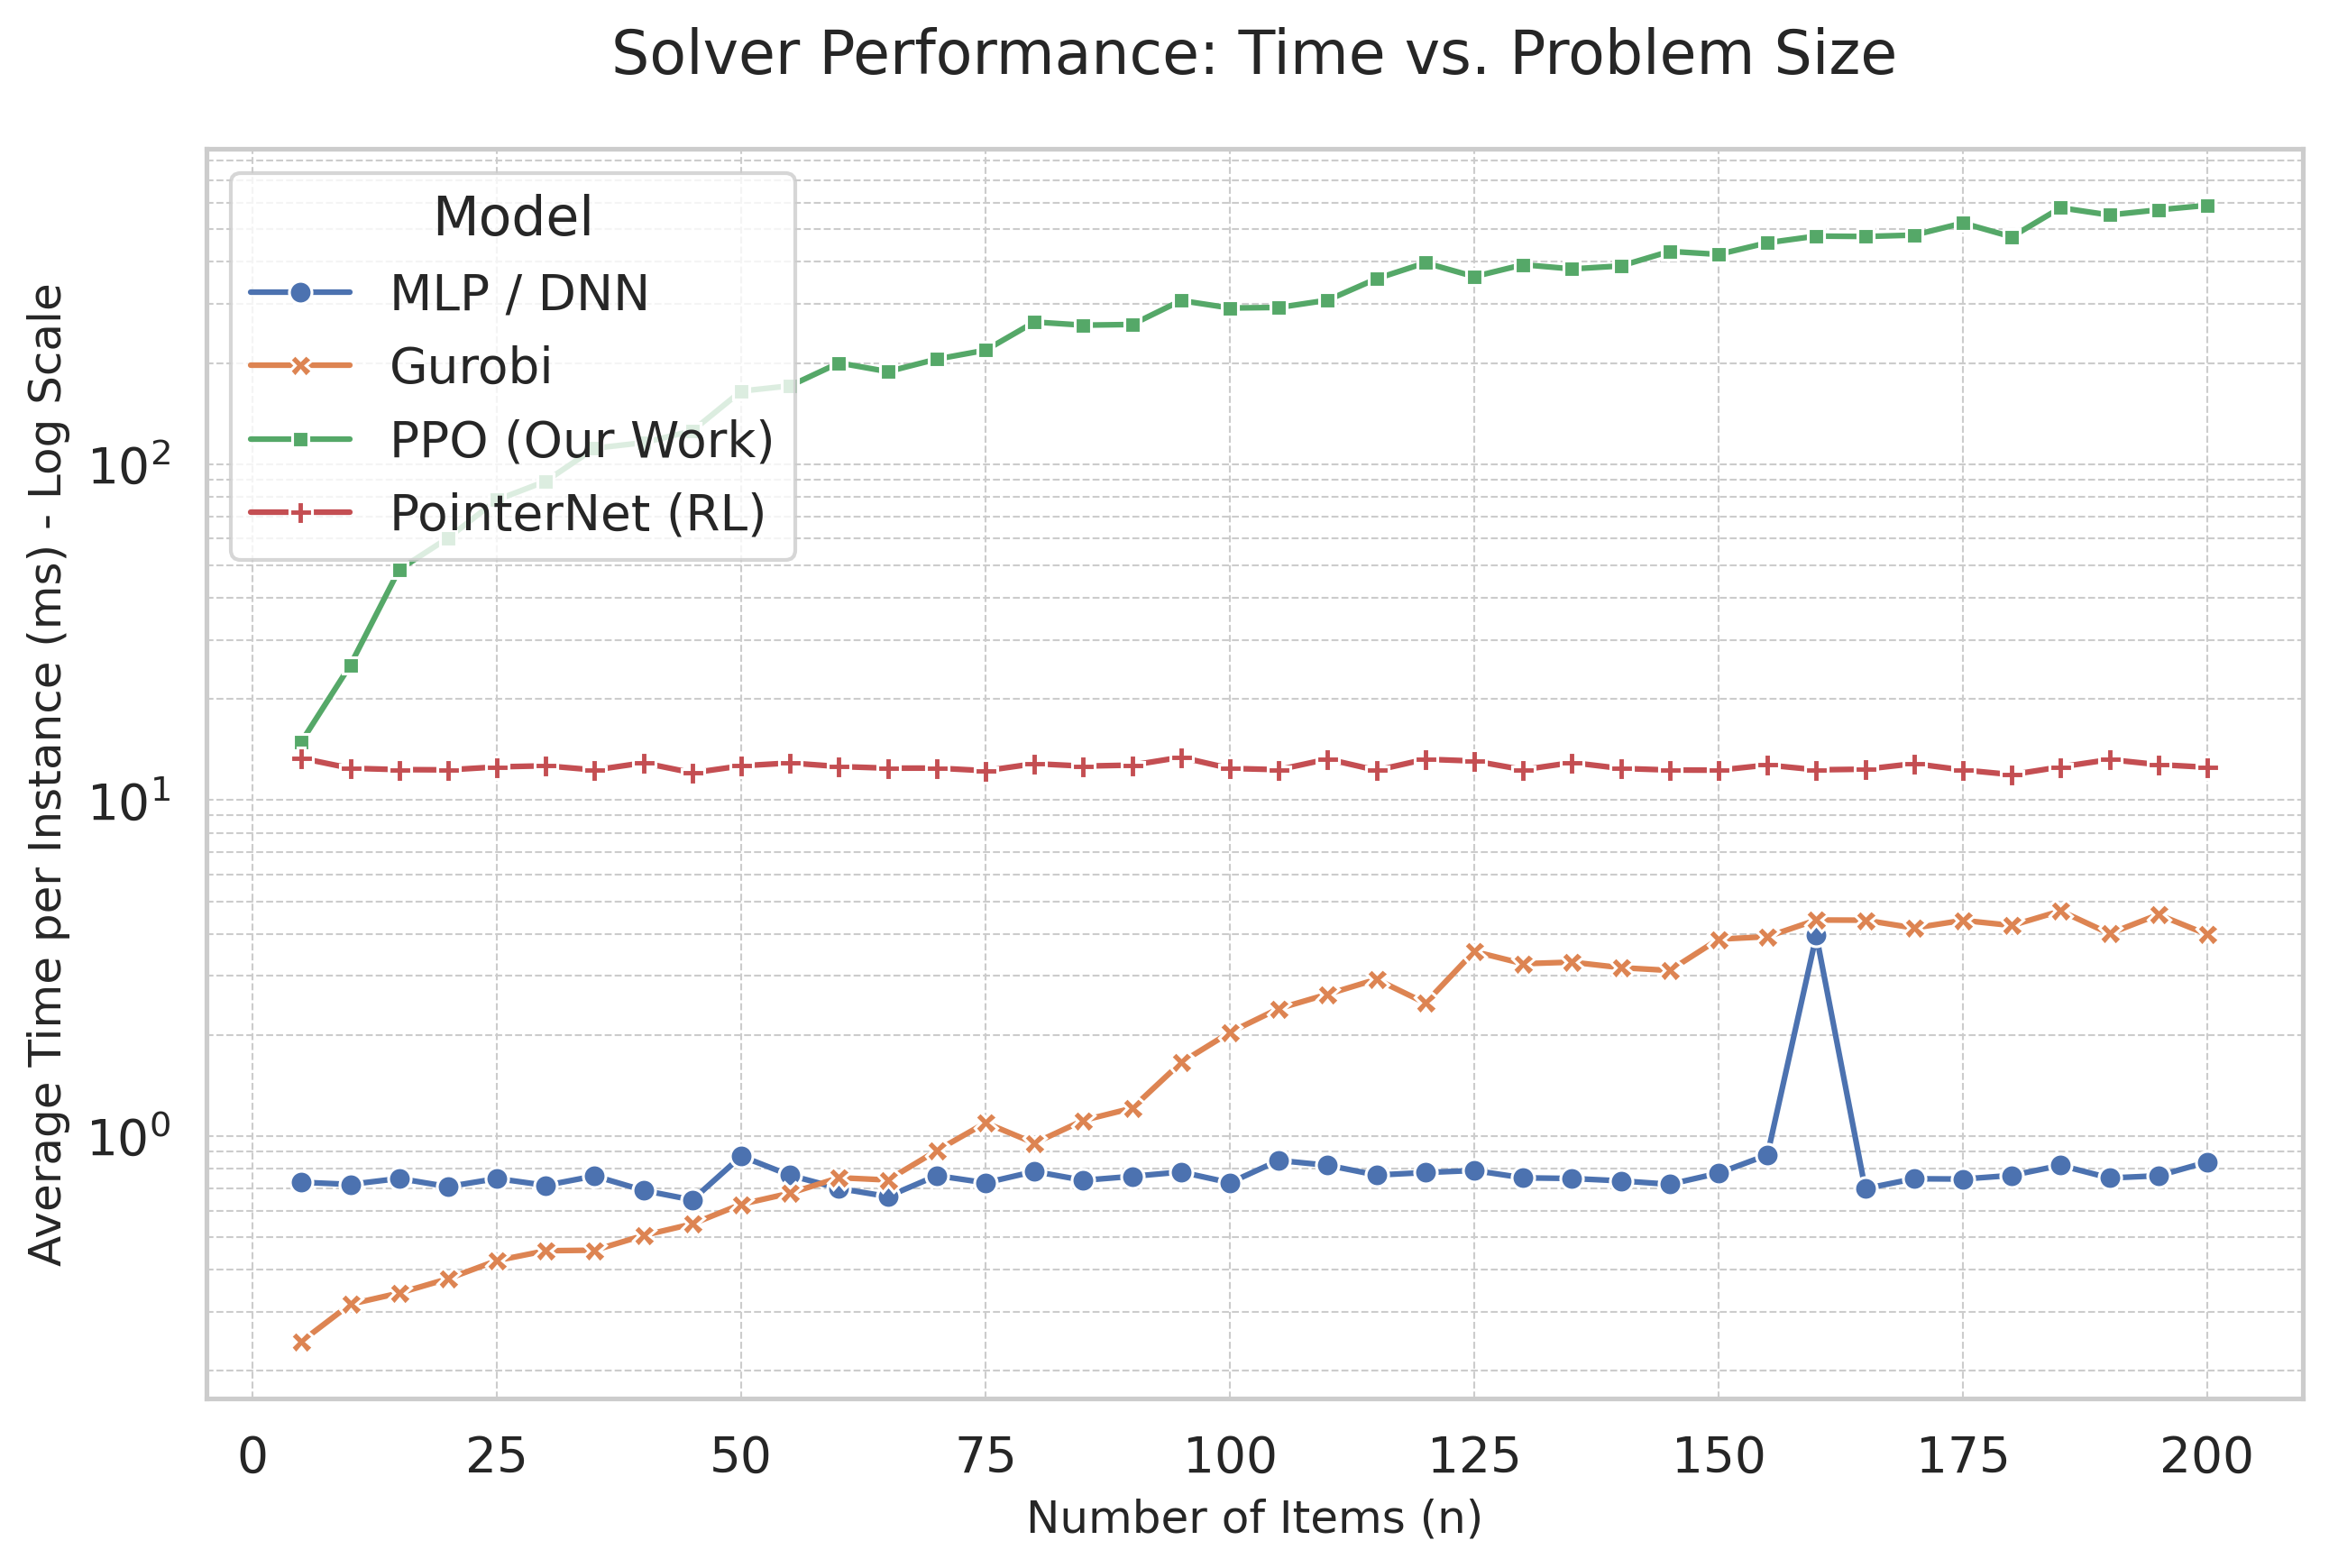
\includegraphics[width=0.48\textwidth]{evaluation_times_vs_n_styled.png}
            \label{fig:time_results}
        }
    \end{figure}
    
    \vspace{-0.6em} % Reduce the space between figures and the text below

    % --- BOTTOM PART: Analysis text in two columns ---
    \begin{columns}[T]
        % --- LEFT COLUMN: Analysis for the MRE plot ---
        \begin{column}{0.5\textwidth}
            \begin{block}{Key Findings: Accuracy}
                \begin{itemize}
                    \item Our PPO model maintains a low Mean Relative Error (MRE), demonstrating high solution quality and strong generalization.
                    \item Pointer Network shows a higher error rate.
                    \item The pure MLP model fails to generalize effectively.
                \end{itemize}
            \end{block}
        \end{column}

        % --- RIGHT COLUMN: Analysis for the Time plot ---
        \begin{column}{0.5\textwidth}
            \begin{block}{Key Findings: Inference Time}
                \begin{itemize}
                    \item PPO's inference time is practical for large instances.
                    \item Pointer Network is faster but less accurate.
                    \item MLP is the fastest but provides poor solutions.
                \end{itemize}
            \end{block}
        \end{column}
    \end{columns}
\end{frame}
% ===================================================================
% SECTION 5: CONCLUSION & FUTURE WORK
% ===================================================================
\section{Conclusion \& Future Work}

% --- Slide 1: Conclusion ---
\begin{frame}
    \frametitle{Conclusion}

    \begin{columns}[T]
        % --- LEFT COLUMN: Performance Summary ---
        \begin{column}{0.5\textwidth}
            \begin{block}{Performance Summary}
                \begin{itemize}
                    \item \textbf{PPO vs. Pointer Network (Accuracy):} \\
                    \begin{itemize}
                        \item \textbf{Algorithmic Superiority:} PPO's Actor-Critic (TD) method provides low-variance updates.
                        \item \textbf{Architectural Advantage:} The \textbf{Transformer} encoder captures the global, combinatorial nature of the problem more effectively than a sequential \textbf{LSTM}.
                        \item \textbf{Framework Robustness:} Leveraging \textbf{Stable Baselines 3} provides key stabilizations like adaptive observation normalization (`VecNormalize`).
                    \end{itemize} \vspace{1em}

                    \item \textbf{PPO vs. Pointer Network (Speed):} \\
                    \begin{itemize}
                        \item \textbf{Core Architecture:} \textbf{Transformer} is more computationally intensive than \textbf{LSTM}.
                        \item \textbf{Model Components:} Extra Critic Network requires extra computation.
                        \item \textbf{Evaluation Method:} Stable\_baseline3 cannot support batch evaluation.
                    \end{itemize} \vspace{1em}                    
                \end{itemize}
            \end{block}
        \end{column}
        
        % --- RIGHT COLUMN: Key Methodological Takeaways ---
        \begin{column}{0.5\textwidth}
            \begin{alertblock}{Effective Training Techniques}
                The success of the framework relies on several key techniques:
                \begin{itemize}
                    \item \textbf{Input Normalization:} \\
                    Normalizing item attributes ($w_i, v_i$) and the knapsack capacity ($C$) is crucial. \vspace{1em}
                    
                    \item \textbf{Observation \& Reward Normalization:} \\
                    Using `VecNormalize` for both observations and rewards stabilizes the learning process significantly. \vspace{1em}
                    
                    \item \textbf{Heuristic Preprocessing:} \\
                    Sorting items by value-density ($v_i / w_i$) before feeding them to the model provides a strong inductive bias and improves performance.
                \end{itemize}
            \end{alertblock}
        \end{column}
    \end{columns}
\end{frame}

% --- Slide 2: Future Work ---
\begin{frame}
    \frametitle{Future Work \& Open Questions}

    \begin{block}{Architectural Exploration}
        \begin{itemize}
            \item \textbf{The "Simple Critic" Anomaly:} \\
            A simple MLP Critic achieved higher accuracy (70\%) than a more complex attention-based head (60\%). Future work should investigate if this is due to optimization challenges or a regularization effect. \vspace{1em}
            
            \item \textbf{Global State Representation (`[CLS]` Token):} \\
            Initial experiments with a `[CLS]` token for global state representation surprisingly decreased performance. This warrants further investigation. \vspace{1em}
            
            \item \textbf{Hyperparameter Tuning:} \\
            While a 3-layer MLP Critic works well, its optimal width and the interplay with network depth remain open questions for further tuning.
        \end{itemize}
    \end{block}

    \begin{alertblock}{Problem Formulation \& Reward Shaping}
        \begin{itemize}
            \item \textbf{Explore Alternative Formulation:} Our model uses a \textbf{"Decision" formulation} (select one from all remaining items). An alternative \textbf{"Selection" formulation} (decide 'take' or 'skip' for items sequentially) could be investigated. \vspace{1em}

            \item \textbf{Advanced Reward Shaping:} For the current "Decision" model, an initial attempt at adding a final shaping reward (to encourage a fuller knapsack) decreased accuracy. Further research into more advanced shaping techniques (e.g., potential-based rewards) is needed.
        \end{itemize}
    \end{alertblock}
\end{frame}


% --- Final Thank You Slide ---
\begin{frame}
    \centering
    \Huge{\textbf{Thank You}}
    \vspace{2em}
    \LARGE{Q \& A}
\end{frame}


\end{document}
